\documentclass{article}
\usepackage{graphicx}
\usepackage[utf8]{inputenc}
\usepackage{amsmath, amssymb, latexsym}

\usepackage{pgfplots}
\usepackage{algorithm}
\usepackage[noend]{algpseudocode}
\usepackage{tikz}
\usepackage{nicefrac}
\usepackage{placeins}
\pgfplotsset{every axis legend/.append style={
at={(0,0)},
anchor=north east}}
\usetikzlibrary{shapes,positioning,intersections,quotes}
\usetikzlibrary{arrows.meta,
                bending,
                intersections,
                quotes,
                shapes.geometric}
                
\definecolor{darkgreen}{rgb}{0.0, 0.6, 0.0}
\definecolor{darkred}{rgb}{0.7, 0.0, 0.0}
\makeatletter
\def\BState{\State\hskip-\ALG@thistlm}
\makeatother
\title{Week 17}
\begin{document}
\pagenumbering{gobble}
\maketitle
\newpage
\pagenumbering{arabic}

\section*{Learning with large datasets}
Taking a low bias algorithm and training it on a large amount of data is one of the greatest approaches to get high performance.

\begin{itemize}
  \item Assume we have a data collection with m = 100,000, 000.
  \item On such a large system, how can we train a logistic regression model?

        $$\theta_j := \theta_j - \alpha \frac{1}{m} \sum_{i=1}^m(h_{\theta}(x^{(i)})- y^{(i)})x_j^{(i)}$$

  \item As a result, for each gradient descent step, you must add up more than 100,000,000 terms.
  \item The first step is to inquire whether we may train on 1000 examples rather than 100 000 000.
  \item Pick a small sample at random. Can you build a system that performs well?
\end{itemize}

~\\
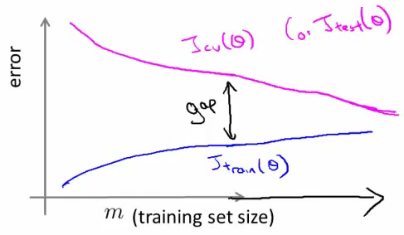
\includegraphics[width=0.5\textwidth]{resources/learning_curve}

\begin{itemize}
  \item If the gap is large, it is a high variance problem. More examples should lead to better results.
  \item If the gap is tiny, it is a high bias problem. More examples may not be beneficial.
\end{itemize}

\section*{Stochastic Gradient Descent}

Hypothesis:
$$h_{\theta}(x) = \sum_{n}^{j=0}\theta_jx_j$$

~\\
Cost function:
$$\quad J_{train}(\theta) = \frac{1}{2m} \sum_{m}^{i=1}(h_{\theta}(x^{(i)}) - y^{(i)})^2$$

~\\
We get bowl shape surface plots if we plot our two parameters against the cost function:

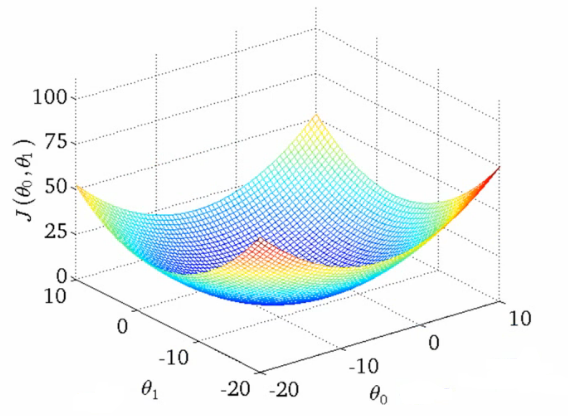
\includegraphics[width=0.5\textwidth]{resources/surface_cost_function}

~\\
How does gradient descent work?

\begin{algorithm}
  \caption{Gradient Descent}\label{euclid}
  \begin{algorithmic}[1]
    \Large
    \While {not converged}
    \State $\theta_j := \theta_j - \alpha \frac{\partial}{\partial \theta_j} J(\theta_0, ..., \theta_n)$
    \State $(for\ j = 0, ..., n)$
    \EndWhile
  \end{algorithmic}
\end{algorithm}

~\\
Although we have just referred to it as gradient descent so far, this type of gradient descent is known as batch gradient descent. This simply implies that we examine all of the examples at the same time. Batch gradient descent is unsuitable for large datasets.

~\\
When discussing stochastic gradient descent, we will use linear regression as an algorithmic example, however the concepts apply to other algorithms as well, such as logistic regression and neural networks.

~\\
Define our cost function in a slightly different way, as follows:
$$\quad J_{train}(\theta) = \frac{1}{m} \sum_{m}^{i=1}cost(\theta, (x^{(i)}, y^{(i)}))$$
$$cost(\theta, (x^{(i)}, y^{(i)}))=\frac{1}{2}(h_{\theta}(x^{(i)}) - y^{(i)})^2$$

\FloatBarrier
\begin{algorithm}
  \caption{Stochastic Gradient Descent}\label{euclid}
  \begin{algorithmic}[1]
    \Large
    \State Randomly shuffle training examples
    \For{\texttt{$i:=1,...,m$}}
    \State \texttt{$\theta_j := \theta_j - \alpha (h_{\theta}(x^{(i)}) - y^{(i)})x_j^{(i)}$}
    \State \texttt{$(for\ j = 0, ..., n)$}
    \EndFor
  \end{algorithmic}
\end{algorithm}
\FloatBarrier

The random shuffling at the start ensures that the data is in a random sequence, preventing bias in the movement.

~\\
Although stochastic gradient descent is similar to batch gradient descent, instead of waiting for the gradient terms to be summed across all m examples, we pick only one example and make work on enhancing the parameters right away.

~\\
This means that we change the parameters on EVERY step through the data, rather than at the end of each loop over all of the data.

~\\
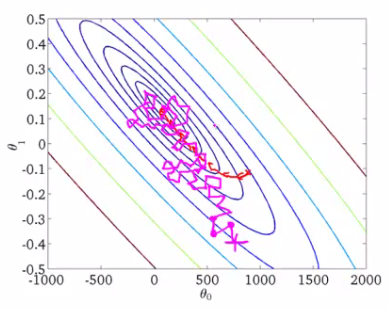
\includegraphics[width=0.6\textwidth]{resources/stochastic}

~\\
For our stochastic gradient descent, we might plot the cost function vs the number of iterations.
We should be able to see if convergence is occurring by looking at the graphs.
A smoother curve may be obtained by averaging across many (e.g. 1000 and 5000) instances.

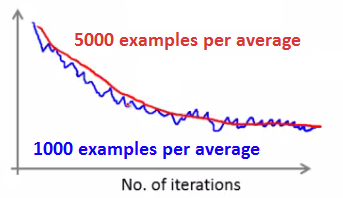
\includegraphics[width=0.45\textwidth]{resources/stochastic_convergence}

\section*{Online learning}

\begin{itemize}
  \item Allows us to model problems in which there is a continuous stream of data from which an algorithm should learn.
  \item In the same way that stochastic gradient descent is used, slow updates are performed.
  \item To learn from traffic, web companies employ several sorts of online learning algorithms.
\end{itemize}

\subsection*{Example - product search}
\begin{itemize}
  \item Assume you own a cellphone-selling website.
  \item You have a user interface where the user may enter in a query such as "Android phone 1080p camera."
  \item We want to provide the user ten phones per query, with the phones ranked from most appealing to the user.
  \item We generate a feature vector (x) for each phone based on a specific user query.
  \item We want to determine the likelihood of a user picking a phone.
  \item $y = 1$ if a user clicks on a link.
  \item $y = 0$ otherwise.
  \item We learn $p(y=1|x;\theta)$ - this is the problem of learning the predicted click through rate (CTR).
  \item If you can estimate the CTR for any phone, we can utilize it to show the phones with the highest likelihood first.
\end{itemize}

\section*{Map reduce and data parallelism}
Some problems are simply too large for a single CPU to handle.

~\\
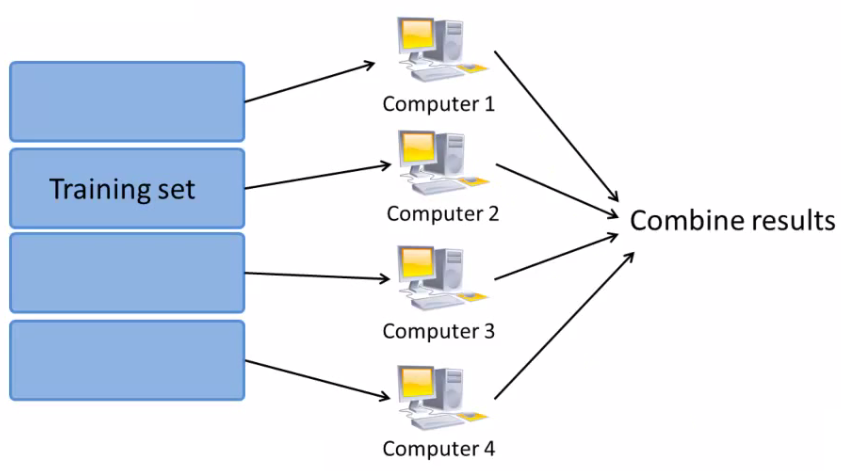
\includegraphics[width=0.6\textwidth]{resources/map_reduce}

Parallelization can come from:
\begin{itemize}
  \item Multiple machines.
  \item Multiple CPUs.
  \item Multiple cores in each CPU.
\end{itemize}

~\\
Certain numerical linear algebra libraries can automatically parallelize your calculations over several cores, depending on the implementation details.
So, if this is the case and you have a decent vectorization implementation, you don't have to worry about local parallelization because the local libraries will handle optimization for you.

~\\
Hadoop is an example of Map Reduce implementation.

\end{document}
